\documentclass[11pt]{article}
\usepackage[margin=1in]{geometry}
\usepackage{graphicx}
\usepackage{amsmath}
\usepackage{booktabs}

\title{A Finite Intercept Correction Calculation}
\author{Anonymous}
\date{}

\begin{document}
\maketitle

\begin{abstract}
This teaching note connects residual arithmetic, fixed-slope least-squares intercept estimation, and error measurement through five synthetic observations. Targets follow $y=2x+3$, while the fixed predictor returns $2x$. Averaging the residuals gives the least-squares correction $b=3$. The recorded corrections $b=0$, $1.5$, and $3$ yield mean squared errors $9$, $2.25$, and $0$. The zero is exact agreement on the observations used to estimate the correction, arising from their constant residuals. An observation table, algebraic decomposition, workflow diagram, and error plot organize the calculation into reproducible steps and distinguish fitting-observation error from error on new observations.
\end{abstract}

\section{Introduction}

This note is intended for introductory learners who can calculate averages and squared errors and are connecting these operations to intercept estimation. Its organizing question is how the same target values enter three operations: forming residuals, estimating an additive correction, and evaluating corrected predictions. The sequence makes these dependencies explicit in a single worked calculation.

The inputs are $x=(-2,-1,0,1,2)$, with targets $y_i=2x_i+3$ and baseline predictions $\hat y_i^{(0)}=2x_i$. Fixing the slope isolates the intercept. Every baseline residual equals $3$, so both the correction and its effect can be checked observation by observation.

The learning objectives are to derive the mean-residual correction, explain why a halfway correction halves absolute error but quarters squared error, and identify which targets supply each reported error. These are mathematical tasks illustrated by the record. The sequence is presented as a worked teaching resource; its claims concern the calculation and its interpretation.

\section{Related Work}

\subsection{Fixed Predictors and Additive Offset Corrections}

Residual averaging here is exactly least-squares intercept estimation with the slope fixed at $2$. Writing predictions as $2x_i+b$ leaves one adjustable quantity. Section~\ref{sec:least_squares} establishes this equivalence directly, making the mathematical background self-contained.

The exposition connects this identity to individual observations and recorded errors. Its organizational emphasis is the passage from a residual vector to a fitted intercept and then to an error calculation.

\subsection{Evaluation of Corrections Estimated from Observed Residuals}

The targets determine both the residual average and the reported errors. We therefore call these errors \emph{fitting-observation errors}: they score the same observations used to estimate $b$. Figure~\ref{fig:residual_workflow} traces this reuse. Agreement on these targets and predictive agreement on new targets are distinct quantities.

\section{Method}

\subsection{Finite Observations and Residual Correction}

Table~\ref{tab:observations} gives the complete record, including the residual used to estimate the correction. For rows $i=1,\ldots,5$, define
\[
r_i=y_i-2x_i,
\qquad
\bar r=\frac{1}{5}\sum_{i=1}^{5}r_i=3.
\]
The fitted correction is $b=\bar r$, giving
$\hat y_i^{\mathrm{corr}}=2x_i+\bar r$.

\begin{table}[htbp]
    \centering
    \caption{Complete observation record. Each residual is the target minus the baseline prediction; adding their mean to the baseline gives the corrected prediction.}
    \label{tab:observations}
    \begin{tabular}{rrrrr}
        \toprule
        \shortstack[r]{Input\\$x_i$} &
        \shortstack[r]{Target\\$y_i$} &
        \shortstack[r]{Baseline\\$2x_i$} &
        \shortstack[r]{Residual\\$y_i-2x_i$} &
        \shortstack[r]{Corrected\\$2x_i+3$} \\
        \midrule
        $-2$ & $-1$ & $-4$ & $3$ & $-1$ \\
        $-1$ & $1$  & $-2$ & $3$ & $1$  \\
        $0$  & $3$  & $0$  & $3$ & $3$  \\
        $1$  & $5$  & $2$  & $3$ & $5$  \\
        $2$  & $7$  & $4$  & $3$ & $7$  \\
        \bottomrule
    \end{tabular}
\end{table}

\subsection{Least-Squares Equivalence and Error Calculation}
\label{sec:least_squares}

The fixed-slope least-squares objective is
\[
L(b)=\frac{1}{5}\sum_{i=1}^{5}(r_i-b)^2.
\]
Writing $r_i-b=(r_i-\bar r)+(\bar r-b)$ and using
$\sum_i(r_i-\bar r)=0$ gives
\[
L(b)=
\underbrace{\frac{1}{5}\sum_{i=1}^{5}(r_i-\bar r)^2}
_{\text{remaining squared error at the optimum}}
+(b-\bar r)^2.
\]
The first term is independent of $b$; the second is uniquely minimized at $b=\bar r$. Thus averaging residuals and fitting the intercept produce the same correction without numerical optimization.

This identity holds for any five residual values. If they differ, at least one squared centered residual is positive, so the minimum error is positive. Exact cancellation occurs precisely when every residual equals their mean. In the supplied record, all equal $3$, giving $L(3)=0$.

For the recorded offsets, the individual errors and their averages are
\[
\begin{aligned}
e_i(b)&=y_i-(2x_i+b)=3-b,\\
\operatorname{MAE}(b)&=\frac{1}{5}\sum_{i=1}^{5}|e_i(b)|=|3-b|,\\
\operatorname{MSE}(b)&=\frac{1}{5}\sum_{i=1}^{5}e_i(b)^2=(3-b)^2.
\end{aligned}
\]

\begin{figure}[htbp]
    \centering
    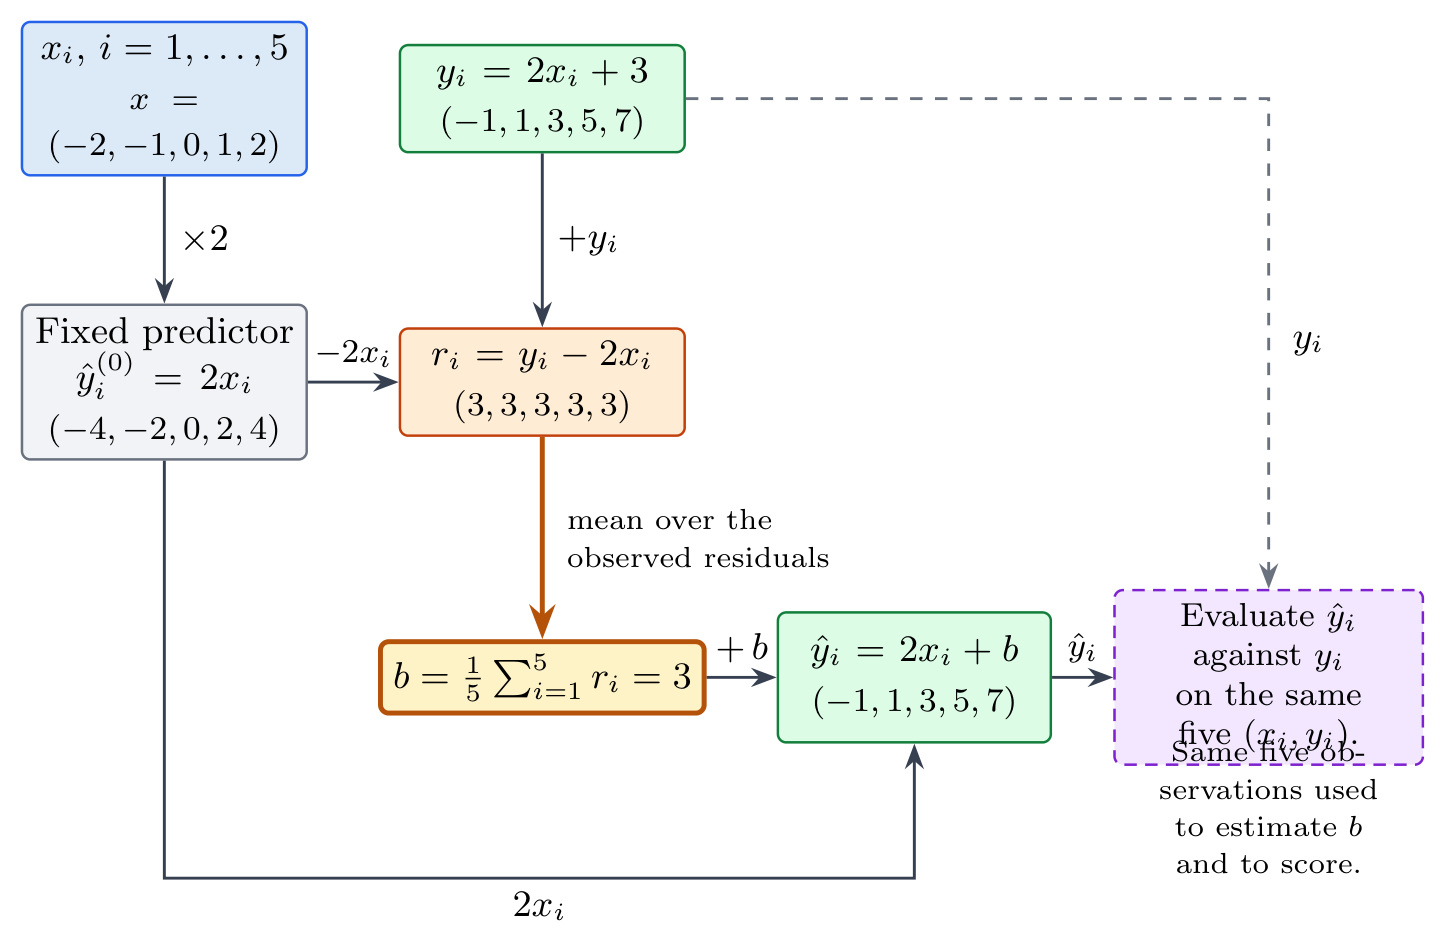
\includegraphics[width=\linewidth]{figures/fig_residual_workflow.jpg}
    \caption{Residual-to-offset workflow. Inputs give baseline predictions $2x_i$; subtracting these from targets gives $(3,3,3,3,3)$. Their mean supplies $b=3$, which is added to the baseline. The corrected predictions are evaluated against the same targets. The direct target-to-evaluation path marks this reuse; the description does not depend on box colors.}
    \label{fig:residual_workflow}
\end{figure}

\section{Experiments}

\subsection{Deterministic Calculation and Recorded Results}

This section reports one deterministic worked calculation in base R. To reproduce it, enter the $x$ and $y$ columns of Table~\ref{tab:observations}, compute \verb|r <- y - 2*x| and \verb|mean(r)|, and evaluate \verb|mean(abs(y - (2*x + b)))| and \verb|mean((y - (2*x + b))^2)| at each recorded offset.

\begin{table}[htbp]
    \centering
    \caption{Recorded fitting-observation errors. All rows use the five observations in Table~\ref{tab:observations}.}
    \label{tab:errors}
    \begin{tabular}{rrr}
        \toprule
        Added intercept $b$ & Mean absolute error & Mean squared error \\
        \midrule
        $0$   & $3$   & $9$    \\
        $1.5$ & $1.5$ & $2.25$ \\
        $3$   & $0$   & $0$    \\
        \bottomrule
    \end{tabular}
\end{table}

The midpoint $b=1.5$ leaves residual $1.5$ at every observation. Relative to $b=0$, MAE is halved and MSE is quartered, illustrating absolute versus squared scaling. The fitted correction $b=3$ produces the corrected column in Table~\ref{tab:observations}.

\subsection{Visualization, Reproducibility, and Interpretation}

The table provides exact values for both metrics; Figure~\ref{fig:intercept_error} displays only the three recorded MSE values. Figure~\ref{fig:residual_workflow} instead identifies the data dependencies.

For self-checking, learners can explain why the residual mean minimizes $L$, why the midpoint gives MSE $2.25$, and whether the scoring targets also determine $b$. The decomposition, Table~\ref{tab:errors}, and workflow respectively supply the answers.

For a new observation $(x_{\mathrm{new}},y_{\mathrm{new}})$, the fitted correction remains $3$, and its error is
\[
e_{\mathrm{new}}
=(y_{\mathrm{new}}-2x_{\mathrm{new}})-3.
\]
Exact cancellation transfers precisely when this new baseline residual equals $3$. New-observation error must therefore be calculated from the new targets; the reported zero describes this constructed fitting record.

\begin{figure}[htbp]
    \centering
    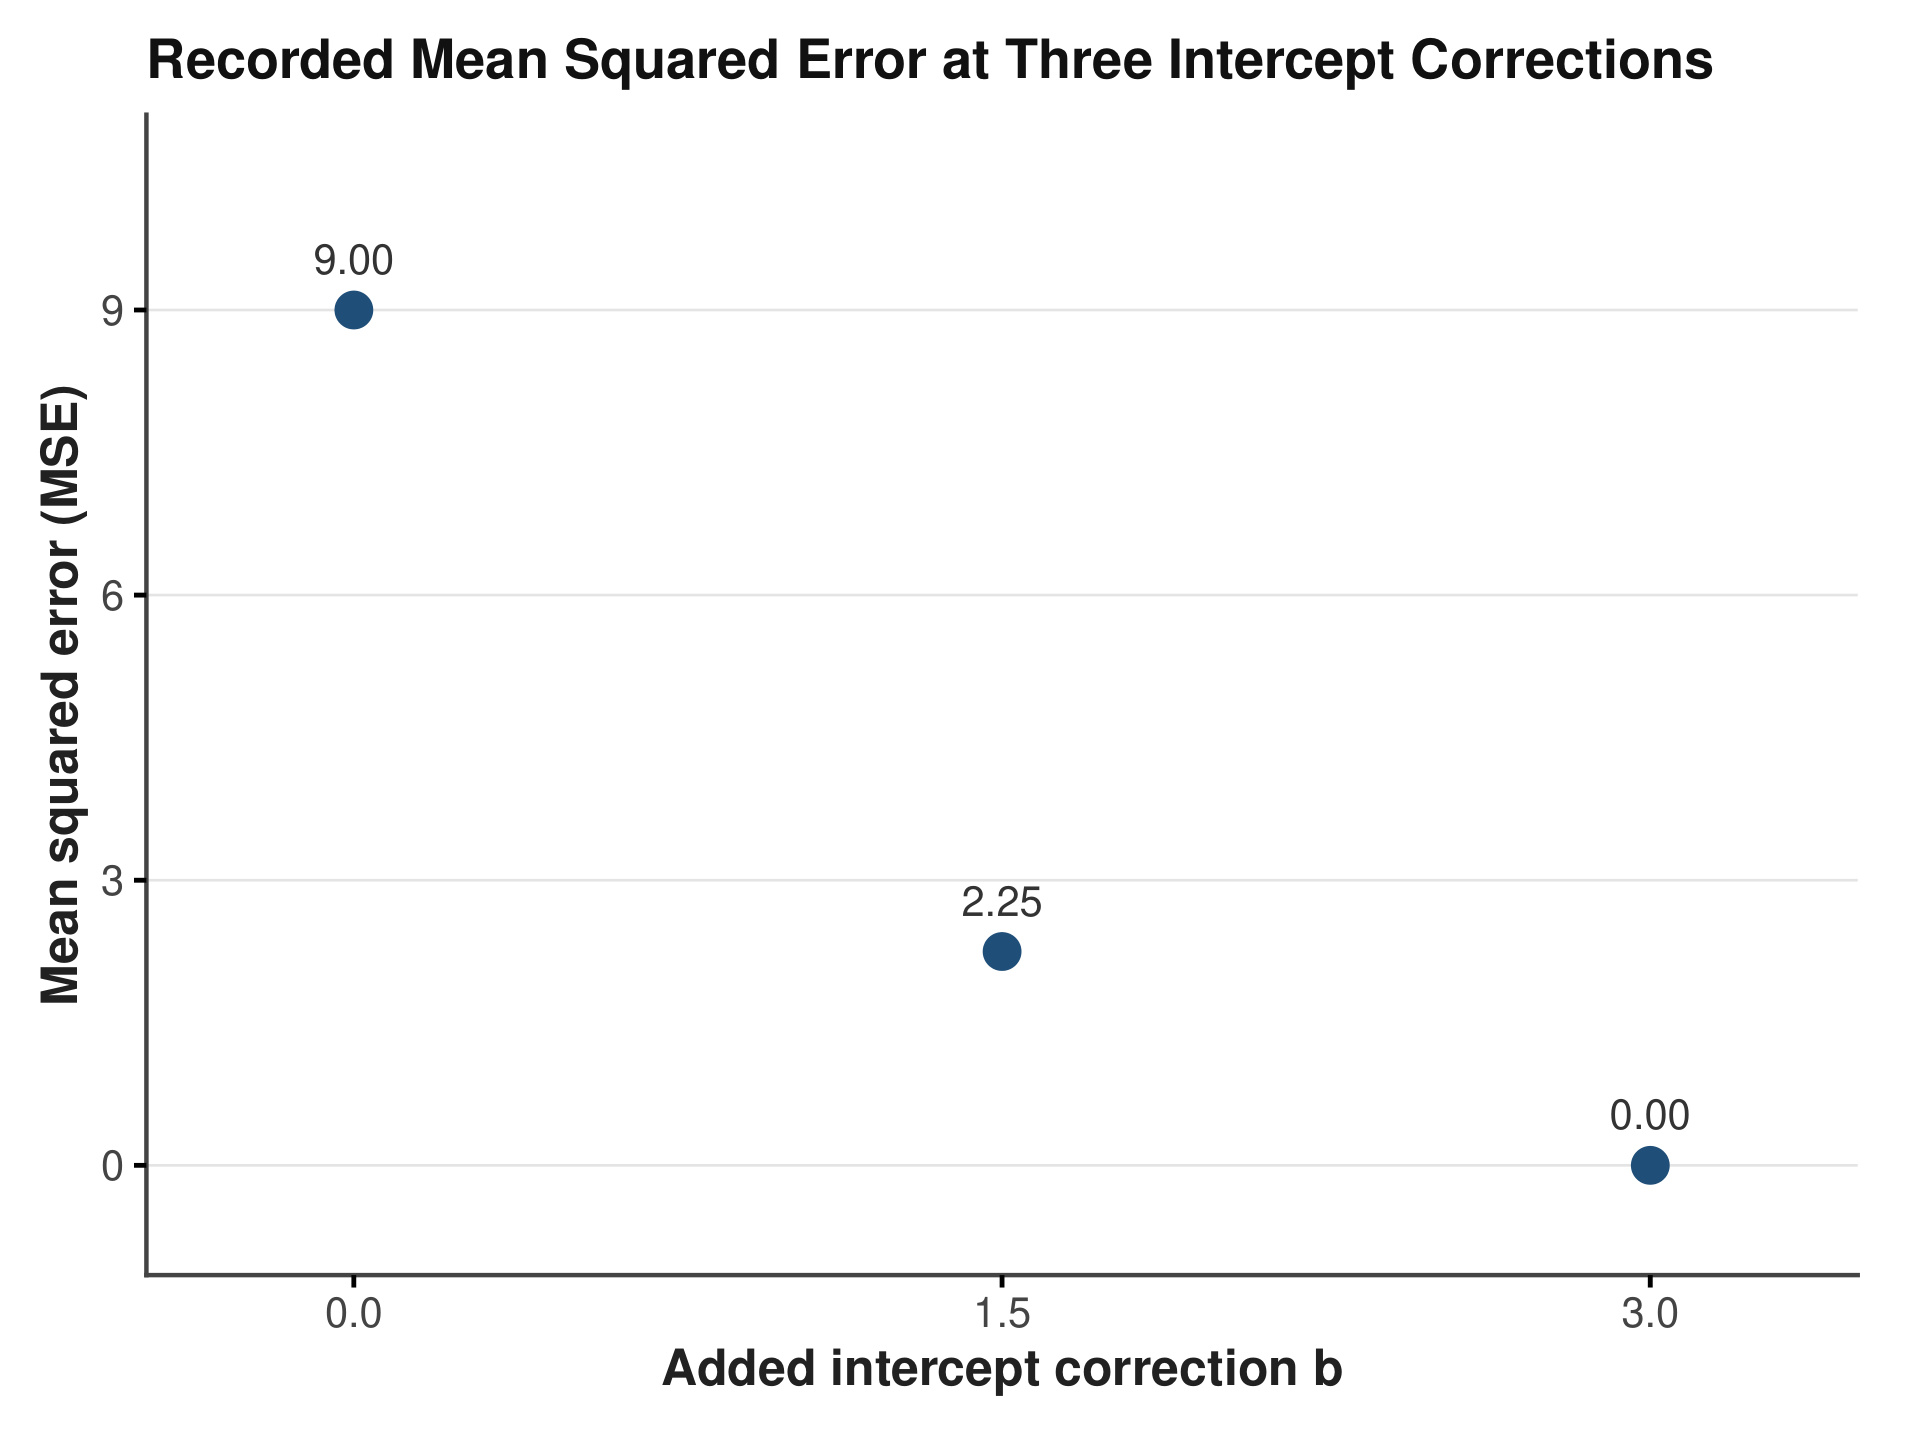
\includegraphics[width=\linewidth]{figures/fig_intercept_error.jpg}
    \caption{Recorded fitting-observation MSE against added intercept $b$. The three labeled points are $(0,9)$, $(1.5,2.25)$, and $(3,0)$. The halfway correction quarters MSE; the fitted correction cancels the common residual. Each point is a recorded value.}
    \label{fig:intercept_error}
\end{figure}

\section{Conclusion}

The worked calculation connects residual averaging, fixed-slope intercept estimation, and error measurement. The decomposition separates minimizing squared error from achieving zero error. Here zero follows from constant residuals on the fitting observations; interpreting predictions on new observations requires their own residuals.

% PAPER_ORCHESTRA_PROVENANCE_BEGIN
\clearpage
\section*{Figure source provenance}
The files below are the exact sources that produced the embedded figure previews. Paths are relative to this manuscript's source directory. The accompanying \texttt{figure\char95{}provenance.json} records all artifact checksums.\par
\medskip\noindent\textbf{Figure~\ref{fig:intercept_error} (\texttt{fig\char95{}intercept\char95{}error.jpg}).}\par
\noindent R/ggplot2 source: \texttt{figure\char95{}code/\allowbreak{}fig\char95{}intercept\char95{}error/\allowbreak{}source.R}.\par
\noindent Source SHA256: \texttt{18933984\allowbreak{}6a19ff9a\allowbreak{}fe13e24a\allowbreak{}7efe95cc\allowbreak{}4a83ec38\allowbreak{}a9778113\allowbreak{}caa8f8c9\allowbreak{}2dd0589a}.\par
\noindent Rendering metadata: \texttt{figure\char95{}code/\allowbreak{}fig\char95{}intercept\char95{}error/\allowbreak{}render.json}.\par
\noindent Exact export wrapper: \texttt{figure\char95{}code/\allowbreak{}fig\char95{}intercept\char95{}error/\allowbreak{}worker.R}.\par
\noindent Wrapper SHA256: \texttt{6cb2b073\allowbreak{}27277f63\allowbreak{}fafbb553\allowbreak{}cd4f1f12\allowbreak{}c0f85bec\allowbreak{}37a49f3f\allowbreak{}a765da16\allowbreak{}a26b58ba}.\par
\noindent Rendering metadata: \texttt{figure\char95{}code/\allowbreak{}fig\char95{}intercept\char95{}error/\allowbreak{}sessionInfo.txt}.\par
\medskip\noindent\textbf{Figure~\ref{fig:residual_workflow} (\texttt{fig\char95{}residual\char95{}workflow.jpg}).}\par
\noindent LaTeX/TikZ source: \texttt{figure\char95{}code/\allowbreak{}fig\char95{}residual\char95{}workflow/\allowbreak{}source.tex}.\par
\noindent Source SHA256: \texttt{4e19b72b\allowbreak{}be6333b3\allowbreak{}602153f3\allowbreak{}eab1b16a\allowbreak{}e392856f\allowbreak{}fa6a5527\allowbreak{}ea378e37\allowbreak{}911eb5fe}.\par
\noindent Rendering metadata: \texttt{figure\char95{}code/\allowbreak{}fig\char95{}residual\char95{}workflow/\allowbreak{}render.json}.\par
% PAPER_ORCHESTRA_PROVENANCE_END
\end{document}